%!TEX root = ../template.tex
%%%%%%%%%%%%%%%%%%%%%%%%%%%%%%%%%%%%%%%%%%%%%%%%%%%%%%%%%%%%%%%%%%%%
%% chapter3.tex
%% NOVA thesis document file
%%
%% Chapter with a short latex tutorial and examples
%%%%%%%%%%%%%%%%%%%%%%%%%%%%%%%%%%%%%%%%%%%%%%%%%%%%%%%%%%%%%%%%%%%%

\typeout{NT FILE chapter3.tex}%

\chapter{Planning}
\label{cha:Planning}

\section{Proposed Timeplan and Workflow}
In this chapter, a time-plan to be followed during the course of this
dissertation is proposed(figure \ref{fig:timeplan}), with a brief description
of each step being presented afterwards.

\begin{figure}[htbp]
	\centering
	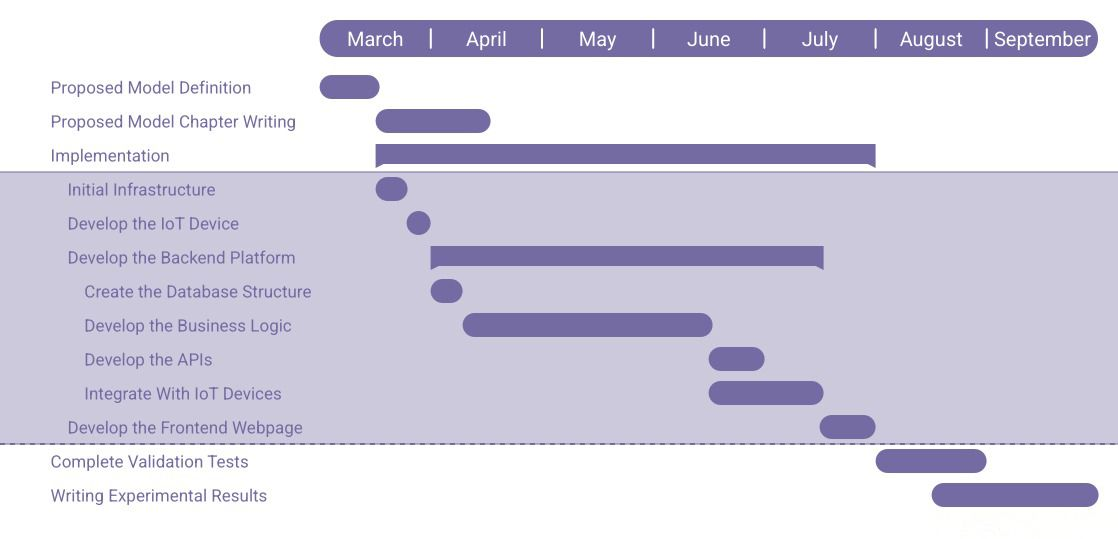
\includegraphics[width=\textwidth]{Chapters/Figures/Planning/Planning.jpeg}
	\caption{Gantt chart with the timeplan proposed}
	\label{fig:timeplan}
\end{figure}

\begin{description}
	\item[Proposed Model Definition:] The system's architecture will be designed
	      over the month of march. The general structure will be defined as well as
	      each component's tech stack and how they communicate.
	\item[Proposed Model Chapter Writing:]  After the model has been established,
	      the proposed model's chapter will be written, describing the architecture
	      in depth as well as its inner components.
	\item[Implementation:] Between April and August, the defined model will be
	      implemented. During this phase, each component will be developed as designed
	      and tested. The test will be done both by unit(unit testing) and to the
	      integration between components(integration testing).
	\item[Writing Experimental Results:] The experimental results will be
	      documented in full in the dissertation in the last two months.
	\item[Revising state-of-the-art:] In the last month, the state-of-the-art
	      chapter will be revised and corrected, and the conclusions will be written.
\end{description}

